
\pagebreak
\section{Input and Output}
Unfortunately MATLAB really falls a bit short in input and output of files.
 Their GUI file importer has improved by leaps and bounds, however.
 We'll explore a couple of different ways for file IO below.

\subsection{File Read/Write}
You can read in user data either from the screen or from files.
 The first can be useful for menu switches, etc.
 The second is obviously useful for data files.

\begin{quote}
\verbatiminput{code/ch05_fileio.m}
\end{quote}

Note: You can also do low-level IO with \emph{fopen}, \emph{fread}, and \emph{fwrite}.
 I would avoid this at all costs, as there is usually a faster way.
 Still, this can be helpful when reading binary files.

\pagebreak
\subsection{GUI File Read}
Matlab can automate the reading of most simple delimited text files.
 You can then copy Matlab code to automate the read later.
 This can only really be demonstrated with screnshots;

\begin{figure}[ht!]
\centering
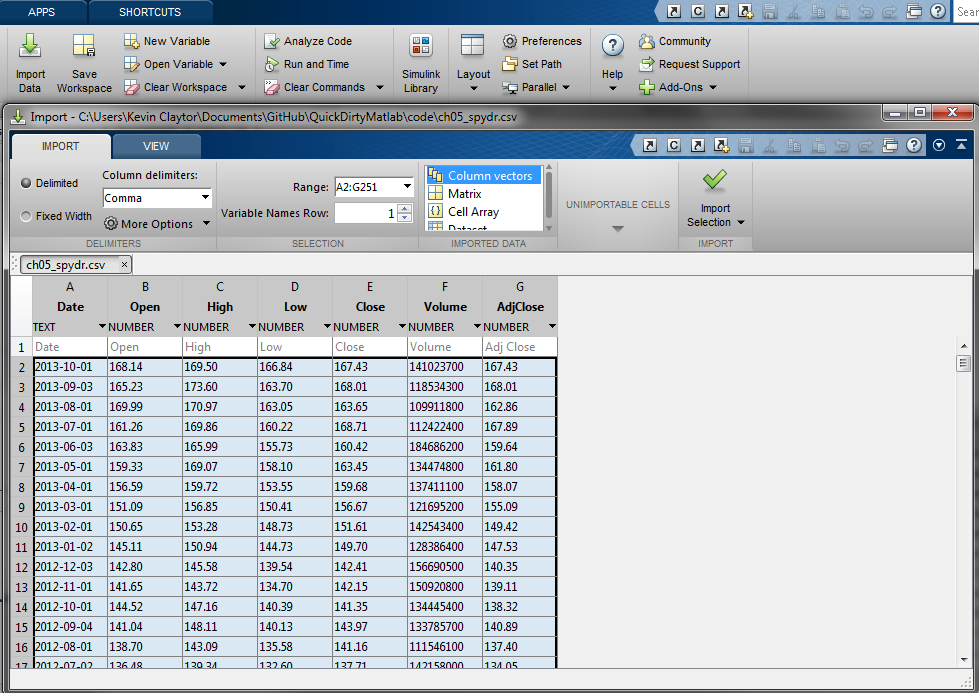
\includegraphics[width=120mm]{img/guiload.png}
\caption{The GUI file reader. From here you can select what subset of your data to import.}
\label{guiload}
\end{figure}

\pagebreak
\subsection{Save and Load}
Matlab also has \emph{save} and \emph{load} commands that allow for direct saving of multiple Matlab variables and variable types.
 This is similar to Python's pickle module.

\begin{quote}
 \verbatiminput{code/ch05_saveload.m}
\end{quote}
